\documentclass{report}

% Graphismes
\usepackage[pdftex]{graphicx}
\usepackage{lmodern}
\usepackage{tikz}
\usepackage{tikz-uml}
\usepackage{pgfgantt}
\usepackage{lscape}
\usepackage{rotating}

% Couleurs personnalisées
\definecolor{matred}{RGB}{239,83,80}
\definecolor{matgreen}{RGB}{156,204,101}
\definecolor{matblue}{RGB}{41,182,246}
\definecolor{matyellow}{RGB}{255,235,59}
\definecolor{matblack}{RGB}{33,33,33}
\definecolor{matgray}{RGB}{224,224,224}
\definecolor{matbrown}{RGB}{78,52,46}

% Packages basiques
\usepackage[utf8]{inputenc}
\usepackage[T1]{fontenc}
\usepackage{lmodern}
\usepackage{geometry}
\usepackage[french]{babel}
\usepackage{hyperref}

% Noms personnalisés
\addto{\captionsfrench}{\renewcommand{\bibname}{Webographie}}

\begin{document}

% Page de garde
\begin{titlepage}
    \centering

    % Titre de la formation
    \textsc{\LARGE Projet L1 -- C.M.I.}\\
    \vspace{.25cm}
    {\Large Spécialité informatique}
    \vspace{3cm}

    % Titre du projet
    \rule{\linewidth}{0.5mm}\\
    \vspace{.4cm}
    {\huge\bfseries Skizzle}\\
    \vspace{.2cm}
    \rule{\linewidth}{0.5mm}
    \vspace{2cm}

    % Author and supervisor
    \begin{minipage}{0.495\textwidth}
        \begin{flushleft}\large
            Maëlle \textsc{Beuret}\\
            Rémi \textsc{Cérès}\\
            Mattéo \textsc{Delabre}
        \end{flushleft}
    \end{minipage}
    \begin{minipage}{0.495\textwidth}
        \begin{flushright}\large
            \textbf{Année :} 2015 -- 2016\\
            \textbf{Soutenu le :} 29/04/2016
        \end{flushright}
    \end{minipage}

    \vfill

    % Logos
    \newcommand{\logo}[2]{
        \raisebox{-.5\height}{
            \includegraphics[scale=#2]{#1}
        }
    }

    \logo{figures/frontpage-logo-um.png}{0.5}
    \logo{figures/frontpage-logo-fds.png}{0.25}
    \logo{figures/frontpage-logo-cgi.png}{0.05}
    \logo{figures/frontpage-logo-figure.png}{1}
\end{titlepage}

% Table des matières
\setcounter{tocdepth}{1}
\tableofcontents

\setlength{\parskip}{0.4cm plus4mm minus3mm}

% Sous-parties
\chapter{Introduction}

Dans le cadre du module Projet C.M.I. du second semestre de L1,
nous avons développé en équipe un jeu vidéo nommé « Skizzle ».
Notre groupe est composé de trois personnes~: Maëlle \textsc{Beuret},
Rémi \textsc{Cérès} et Mattéo \textsc{Delabre}.

L'objectif de ce projet est la création d'un jeu vidéo fonctionnel.
Le jeu mobilise les bases d'algorithmique apprises au premier semestre ainsi
que nos connaissances et recherches personnelles. La création de ce jeu nous
a permis de renforcer nos capacités de travail en collaboration, en
communication et en gestion de projet en général.

Le développement du projet s'est déroulé sur une période d'un mois
et une semaine~: du vendredi 4 mars 2016 au lundi 11 avril 2016 inclus.
Chaque vendredi, lors de la séance de trois heures consacrée au projet,
les trois membres de l'équipe se réunissent pour résumer le travail effectué
la semaine passée et planifier celui de la semaine à venir.

\section{Choix du jeu}

Nous avons d'abord réalisé une étude comparative entre trois jeux
vidéos possibles. Pour ces jeux vidéos, le choix était libre. Notre choix
s'est porté sur un jeu avec un principe original inspiré des jeux de
plates-formes, de coopération et de réflexion. Nous l'avons appelé
« Skizzle », à mi-chemin entre l'anglais \emph{skill} et \emph{puzzle.}

Le jeu se joue à deux joueurs. Chaque joueur est affecté à une balle qu'il
contrôle par le clavier. Le but est pour ces joueurs de faire traverser leur
balle à travers des niveaux prédéfinis. Pour ce faire, les joueurs doivent
utiliser différents phénomènes physiques et constructions mises en place
à la fois dans le niveau et dans le moteur physique du jeu.

Les niveaux se présentent sous la forme de casse-têtes courts à difficulté
progressive. Les deux joueurs doivent souvent réfléchir et s'entraider
pour pouvoir parvenir à la fin. Ce n'est que lorsque les deux joueurs
franchissent la ligne d'arrivée que la partie est gagnée.

\section{Cahier des charges}

Le jeu doit fonctionner sur tous les systèmes courants (Linux, OS X, Windows).
À l'ouverture du jeu, un menu doit permettre d'orienter le joueur vers
les différents états de jeu disponibles, notamment le jeu ou l'éditeur.
Avant d'ouvrir le jeu, on doit pouvoir choisir le niveau à jouer. Avant
d'ouvrir l'éditeur, on doit pouvoir choisir le niveau à éditer ou si l'on
veut créer un nouveau niveau.

Le jeu se joue à deux joueurs qui incarnent chacun une balle contrôlable au clavier.
Une partie doit se présenter sous la forme d'un niveau où les joueurs
ont une position initiale et une position à atteindre pour gagner.
Chaque partie est limitée en temps. La durée limite est définie selon le niveau.

Les mécanismes physiques à implémenter sont la force d'attraction chargée
(coulombienne), la force de gravité, les forces de frottement et les
collisions entre objets. La force de gravité est appliquée selon un vecteur
de norme constante mais de direction et sens modifiables selon les
conditions du niveau.

La caméra des joueurs doit être centrée sur la position intermédiaire
des deux joueurs et doit s'orienter dans la direction inverse
de la direction actuelle de la gravité, en tout temps.

Chaque niveau est composé d'objets. Chaque objet possède une masse,
un coefficient de frottement statique et dynamique, un coefficient
de restitution, une charge, une position, une vitesse et un calque d'affichage
(couche). Un objet est soit une balle d'un joueur soit un bloc. Un bloc
peut être neutre ou posséder une particularité.
Les blocs particuliers sont définis complètement dans la section
\ref{sec:manuel-objets}.

Dans chaque niveau est définie une zone de jeu. Cette zone est un polygone
contrôlé par un nombre arbitraire de points. Si un objet avec une masse
non-infinie se trouve en dehors de cette zone (notamment un joueur
ou bien un bloc déplaçable), il doit être immédiatement tué. S'il s'agissait
d'un joueur, la partie se termine.

Les niveaux doivent être éditables par un éditeur. L'éditeur permet
de créer un nouveau niveau ou d'éditer un niveau existant. Il permet
de placer des objets prédéfinis sélectionables depuis la barre d'outils.
Il permet notamment de situer les positions initiales des joueurs
et du(des) bloc(s) d'arrivée. On doit pouvoir modifier la polarité des objets
depuis l'éditeur. Le niveau modifié doit pouvoir être sauvegardé. On doit
pouvoir tester le niveau en cours d'édition depuis l'éditeur sans perdre
son travail. On doit pouvoir modifier la taille de la zone de jeu.

\chapter{Organisation du projet}

\section{Organisation du travail}

Chaque membre du groupe a travaillé en autonomie. Les réunions lors des séances
prévues étaient consacrées aux explications sur le travail de chacun ainsi qu'à
la répartition des tâches pour la semaine suivante.

Chacun d'entre nous était chargé de tâches spécifiques (voir figure 2.1).
Certaines parties du développement nécessitaient plusieurs personnes et
étaient ainsi partagées entre certains membres du groupe. La conception
et les tests des niveaux, le fond des menus ainsi que les décors furent
réalisés par Rémi et Maëlle, et la gestion de projet par tout le groupe.

Tout au long de la réalisation du projet, nous communiquions par Skype
afin de s'informer de l'avancement et réfléchir à des solutions lorsqu'un
problème était rencontré.

\newgeometry{left=2cm,top=1.5cm,bottom=1.5cm,right=2cm}
\begin{figure}[p!]
    \centering
    \begin{gantt}{32}{32}
    \begin{ganttitle}
        \titleelement{Semaine 1 : 04/03 - 10/03}{4}
        \titleelement{Semaine 2 : 11/03 - 17/03}{4}
        \titleelement{Semaine 3 : 18/03 - 24/03}{4}
        \titleelement{Semaine 4 : 25/03 - 31/03}{4}
        \titleelement{Semaine 5 : 01/04 - 08/04}{4}
        \titleelement{Semaine 6 : 09/04 - 15/04}{4}
        \titleelement{Semaine 7 : 16/04 - 22/04}{4}
        \titleelement{Semaine 8 : 23/04 - 29/04}{4}
    \end{ganttitle}

    \ganttgroup{Moteur physique}{0}{14}
    \ganttbar[color=red]{Organisation des classes}{0}{6}
    \ganttbar[color=green]{Gestion de l'affichage}{0}{8}
    \ganttbar[color=red]{Implémentation des forces}{0}{8}
    \ganttbar[color=red]{Gestion des collisions}{4}{10}
    \ganttbar[color=cyan]{Tests du moteur}{4}{10}

    \ganttgroup{Niveaux du jeu}{6}{26}
    \ganttbar[color=cyan]{Définition du format de fichier}{6}{2}
    \ganttbar[color=red]{Lecture et écriture du format}{12}{4}
    \ganttbar[color=red]{Création de l'éditeur}{16}{5}
    \ganttbar[color=red]{Blocs spécialisés}{18}{3}
    \ganttbar[color=cyan]{Niveau de test}{19}{2}
    \ganttbar{Conception des niveaux}{19}{13}
    \ganttbar{Tests des niveaux}{19}{13}

    \ganttgroup{Interface du jeu}{10}{22}
    \ganttbar[color=red]{Découpage en états de jeu}{10}{4}
    \ganttbar[color=green]{Création du menu}{12}{6}
    \ganttbar[color=red]{Interface de l'éditeur}{16}{5}
    \ganttbar[color=red]{Menus gagné, perdu, pause}{24}{8}

    \ganttgroup{Univers graphique}{8}{20}
    \ganttbar[color=green]{Création des musiques}{8}{8}
    \ganttbar{Fond du menu}{12}{8}
    \ganttbar{Décor}{14}{7}
    \ganttbar[color=cyan]{Textures blocs}{18}{3}
    \ganttbar[color=red]{Implémentation décor}{24}{4}

    \ganttgroup{Gestion de projet}{21}{11}
    \ganttmilestone{Rendu du code}{21}
    \ganttbar{Rédaction du rapport}{21}{4}
    \ganttmilestone{Rendu du rapport}{25}
    \ganttbar{Tests pré-présentation}{25}{7}
    \ganttmilestone{Présentation du jeu}{32}
\end{gantt}

    \caption{
        Diagramme de la répartition des tâches. En vert, les tâches
        affectées à Maëlle~; en bleu, les tâches affectées à Rémi~;
        en rouge, les tâches affectées à Mattéo~; en gris, les
        tâches résolues en groupe
    }
    \label{fig:organisation-gantt}
\end{figure}
\restoregeometry

\section{Outils de développement}

Nous avons choisi le C++ tout d'abord car il s'agit du langage que nous
apprenons cette année, ensuite car il possède de nombreuses bibliothèques.
C'est un langage très utilisé dont le code est élégant. Parmi les bibliothèques
graphiques, nous avons choisi la SFML car son utilisation est simple et
elle correspondait bien à nos besoins.

Pour écrire le code, nous avons utilisé différents éditeurs de texte
(atom et gedit). Nous compilions notre programme avec g++. Pour faciliter
la compilation, nous avons utilisé CMake.

Git nous a permis de gérer les versions du programme, avec le gestionnaire
de projet GitHub, où nous déposions le code ainsi que les documents tels
que le diagramme UML de classes permettant de s'y retrouver plus facilement
dans les nombreuses classes que nous avons créées.

\chapter{Analyse du projet}

\section{Découpage du projet}

Le jeu est constitué d'une suite de niveaux organisés de manière
semblable à ceux d'un jeu de plateformes. Ces niveaux contiennent des entités.

Les entités du jeu sont multiples : blocs, blocs spéciaux, joueurs,
éléments de décor. Ces entités -- ou objets, interagissent entre elles
par un certain nombre de phénomènes physiques « naturels ». Pour répondre
à ce besoin, \textbf{un moteur physique} est nécessaire. Le moteur physique est
chargé de gérer les forces s'appliquant aux objets du jeu, de répondre
aux collisions entre objets et de faire évoluer les objets en conséquence
des forces qui leur sont appliquées.

Plusieurs moteurs physiques en 2D existent déjà dans le langage que nous
avons choisi, notamment Box2D. \cite{analyse-box2d}
Nous avons choisi d'implémenter le moteur
physique du jeu par nous-mêmes pour répondre aux besoins particuliers
(notamment la force d'attraction) et car cela nous permet de mettre en
pratique les savoirs acquis au premier semestre dans le module
de physique générale.

Les \textbf{niveaux du jeu} sont constitués de ces entités et d'autres
métadonnées. Pour pouvoir éditer les niveaux, les sauvegarder et
y rejouer plus tard, il est nécessaire de pouvoir les stocker
en dehors de la mémoire. Nous avons pour ce faire choisi de définir
un format de fichier binaire permettant leur stockage sur le disque.
Des fonctions pour coder et décoder ce format devront être écrites.

Skizzle propose différents \textbf{états de jeu}, notamment, on peut à tout moment
se trouver dans l'éditeur, dans le jeu en lui-même ou sur la vue des règles.
Pour pouvoir accéder à ces états, nous devons créer un menu. L'ensemble
des états du jeu doit être abstrait pour pouvoir être géré dans la classe
principale. Certains états du jeu proposeront des éléments interactifs
(boutons, barres d'outils, zones de texte) qui doivent être implémentés.

Enfin, les différents \textbf{objets du jeu} sont représentés à l'écran en
dessinant des textures. Nous avons également choisi d'ajouter des musiques
au jeu pour le rendre plus convivial. D'autres éléments graphiques doivent
être créés, par exemple le fond du menu. Tous ces éléments sont regroupés
dans l'univers graphique du jeu.

\section{Découpage du code}

Nous avons choisi d'organiser notre code selon le paradigme objet. La plupart
du code est sorti en dehors du \texttt{main}, dont la seule fonction est d'instancier
la classe \texttt{Manager} qui gère de manière abstraite le jeu et de démarrer
le premier état du jeu~: le menu.

\subsection{États, gestion des états et des ressources}

Un état du jeu modélise un écran pouvant être affiché. Une classe
abstraite \texttt{State} chapeaute toutes les classes d'états et permet
de requérir l'implémentation d'une interface commune~:

\begin{itemize}
    \item \texttt{enable()}~: cette méthode initialise l'état avant qu'il
    commence à être affiché. L'état implémentant cette méthode doit
    mettre en place les ressources globales utilisées comme la lecture
    de la musique, le titre de la fenêtre, les éléments de l'interface
    quand cette méthode est appelée~;

    \item \texttt{processEvent(event)}~: cette méthode est appelée avec
    un événement lorsque celui-ci est extrait par la SFML lors de la boucle
    principale. L'état est censé décider s'il souhaite traiter cet événement
    et, si oui, modifier ses variables en conséquence~;

    \item \texttt{frame()}~: cette méthode est appelée lorsque l'état
    doit dessiner une frame à l'écran. Pour éviter d'encombrer la boucle
    principale, l'état doit dessiner sa frame le plus rapidement possible.
\end{itemize}

Les états suivants sont implémentés et descendent de la classe \texttt{State}~:
\texttt{Rules} pour afficher les règles du jeu, \texttt{Menu} pour afficher
le menu du jeu, \texttt{Level} pour afficher les niveaux (soit l'éditeur,
soit le jeu en lui-même).

On définit \texttt{Manager} la classe qui gère les éléments principaux du jeu.
Notamment, \texttt{Manager} maintient une pile d'états qui est initialisée
contenant une seule instance de la classe \texttt{Menu} et peut être
empilée ou dépilée par les états. Par exemple, le menu peut empiler
un nouvel état instance de \texttt{Rules} pour « démarrer » la vue affichant
les règles. En tout temps, l'état en haut de la pile est celui qui est actif
(il reçoit les événements et est dessiné).

La librairie SFML permet de charger les ressources comme la musique,
les images et les polices. Cependant, recharger ces ressources à chaque
utilisation serait inefficace. La classe \texttt{ResourceManager} permet
de mutualiser ces ressources~: les états lui demandent les ressources
à obtenir et le gestionnaire de ressources s'arrange pour ne charger
la ressource qu'à la première demande et à la garder en mémoire par la suite.
Le gestionnaire des ressources mutualise l'accès aux polices, textures
et à la lecture de la musique.

La figure \ref{fig:analyse-uml-state} résume les classes de gestion
d'états et de ressources présentées.

\newgeometry{left=1cm,top=2cm,bottom=2cm,right=1cm}
\begin{figure}[p!]
    \centering
    \begin{tikzpicture}
    %%%%%%%%%%%%%%%%%%%%%%%
    %% CLASSES GÉNÉRALES %%
    %%%%%%%%%%%%%%%%%%%%%%%

    % Spécifications du gestionnaire de jeu
    \umlclass{Manager}{
        window : fenêtre\\
        resource\_manager : \texttt{ResourceManager}\\
        clock : horloge\\
        states : pile de \texttt{State}
    }{
        start() : vide\\
        pushState(state : \texttt{State}) : vide\\
        popState() : vide
    }

    % Spécifications du gestionnaire de ressources
    \umlclass[x=4,y=-4.5]{ResourceManager}{
        textures : dictionnaire \texttt{string -> texture}\\
        fonts : dictionnaire \texttt{string -> police}
        music : musique
    }{
        getTexture(name : string) : texture\\
        getFont(name : string) : texture\\
        getLevelPath(name : string) : string\\
        playMusic(name : string) : vide\\
        stopMusic() : vide
    }
    \umluniassoc{Manager}{ResourceManager}

    % Spécfications d'un état de jeu
    \umlabstract[x=-4,y=-4.5]{State}{
        manager : \texttt{Manager}
    }{
        \umlvirt{enable() : vide}\\
        \umlvirt{processEvent(event : événement) : vide}\\
        \umlvirt{frame() : vide}
    }
    \umlunicompo{Manager}{State}

    %%%%%%%%%%%%%%%%%%%%%%%%%%%%%
    %% ÉTATS DE JEU PRINCIPAUX %%
    %%%%%%%%%%%%%%%%%%%%%%%%%%%%%

    % Spécifications de l'état de jeu abstrait "niveau"
    % qui est une collection d'objets
    \umlabstract[x=7,y=-11]{Level}{}{
        \emph{Voir la figure suivante}
    }
    \umlinherit{State}{Level}

    %%%%%%%%%%%%%%%%%%%%%%%%%%
    %% ÉTATS DE JEU DU MENU %%
    %%%%%%%%%%%%%%%%%%%%%%%%%%

    % Spécifications de l'état de jeu "menu"
    % qui est le premier état au démarrage et permet
    % d'afficher les différents choix de jeu
    \umlclass[y=-11]{Menu}{
        background : sprite\\
        choices : \texttt{[string]}\\
        actions : \texttt{[callback]}\\
        selection : entier non-signé
    }{
        loadMainMenu() : vide\\
        loadLevelMenu() : vide\\
        loadEditorMenu() : vide\\
        launchGame(path : string) : vide\\
        launchEditor(path : string) : vide\\
        launchRules() : vide\\
        quit() : vide\\
        enable() : vide\\
        processEvent(event : événement) : vide\\
        frame() : vide
    }
    \umlinherit{State}{Menu}

    % Spécifications de l'état de jeu "règles" qui
    % affiche l'image décrivant les règles
    \umlclass[x=-7,y=-11]{Rules}{
        background : sprite\\
    }{
        processEvent(event : événement) : vide\\
        frame() : vide
    }
    \umlinherit{State}{Rules}
\end{tikzpicture}

    \caption{Gestion des états et des ressources dans le jeu}
    \label{fig:analyse-uml-state}
\end{figure}
\restoregeometry

\subsection{Niveau et objets}

La classe \texttt{Level} définit les niveaux, qui sont des collections
d'objets. Elle définit la méthode pour dessiner tous les objets d'un niveau,
le charger, le sauvegarder dans un fichier, ajouter ou supprimer des objets.
Elle ne définit pas la méthode \texttt{frame()} que tous les états doivent
implémenter, elle n'est donc pas un état en tant que tel.

Deux classes dérivent de \texttt{Level} : \texttt{Game} pour jouer aux
niveaux et \texttt{Editor} pour les éditer. L'abstraction en
\texttt{Level} permet d'éviter la duplication de code notamment en
ce qui concerne la gestion des objets contenus.

Les classes de niveaux manipulent des collections d'objets. Les objets
modélisent toutes les entités du jeu : les joueurs, les blocs et les
blocs spéciaux. Une classe abstrait les fonctionnalités de tous les objets,
\texttt{Object}.

Les classes \texttt{Block}, définissant l'apparence et le comportement
des blocs, et \texttt{Player}, définissant l'apparence et le comportement
des joueurs, descendent directement d'\texttt{Object}. Enfin, on définit
des blocs spéciaux, qui peuvent réaliser des actions particulières~:

\begin{itemize}
    \item le bloc de gravité modifie la direction de la gravité
    dans un niveau lorsqu'une entité entre en contact avec lui.
    Il ne peut être activé qu'une seule fois par partie~;

    \item le bloc changeur échange la polarité de l'entité
    entrant en contact avec lui. Il ne peut être activé qu'une seule
    fois par partie~;

    \item le bloc tueur tue le joueur entrant en contact avec lui
    et fait perdre la partie (le niveau passe en mode « perdu »)~;

    \item le bloc d'arrivée tue le joueur entrant en contact et lorsqu'il
    ne reste plus de joueurs fait gagner la partie (le niveau passe
    en mode « gagné »).
\end{itemize}

La figure \ref{fig:analyse-uml-level} résume les classes de niveaux
et d'objets.

\newgeometry{left=1cm,top=2cm,bottom=2cm,right=1cm}
\begin{figure}[p!]
    \centering
    \begin{tikzpicture}
    %%%%%%%%%%%%%%%%%%%%%%%%%%%%%
    %% ÉTATS DE JEU PRINCIPAUX %%
    %%%%%%%%%%%%%%%%%%%%%%%%%%%%%

    % Spécifications de l'état de jeu abstrait "niveau"
    % qui est une collection d'objets
    \umlabstract{Level}{
        name : string\\
        background : sprite\\
        music : string\\
        camera : vue\\
        gravity\_direction : direction\\
        total\_time : entier\\
        players : \texttt{[Player]}\\
        objects : \texttt{[Object]}\\
        zone : \texttt{[vecteur]}
    }{
        enable() : vide\\
        processEvent(event) : vide\\
        load(file : string) : vide\\
        save(file : string) : vide\\
        \umlvirt{frame() : vide}\\
        draw() : vide\\
        addObject(object : \texttt{Object})\\
        removeObject(object : \texttt{Object})
    }

    % Spécifications de l'état de jeu "éditeur" qui permet
    % de modifier des niveaux de jeu
    \umlclass[x=-6]{Editor}{
        selection : \texttt{[Object]}
    }{
        enable() : vide\\
        processEvent(event) : vide\\
        frame() : vide\\
        select(objet: \texttt{Object}) : vide\\
        selectAll() : vide\\
        clearSelection() : vide\\
    }
    \umlinherit{Level}{Editor}

    % Spécifications de l'état de jeu "jeu" qui permet
    % de jouer aux niveaux créés
    \umlclass[x=6]{Game}{
        mode : mode\\
        next\_frame\_time : temps\\
        pending\_kill : \texttt{[Object]}\\
        time\_left : flottant
    }{
        enable() : vide\\
        processEvent(event) : vide\\
        frame() : vide\\
        update() : vide\\
        kill(objet : \texttt{Object}) : vide
    }
    \umlinherit{Level}{Game}

    % Spécifications des objets du jeu
    \umlabstract[y=-6.5]{Object}{
        acceleration : vecteur\\
        velocity : vecteur\\
        position : vecteur\\
    }{
        \umlvirt{getForces(game : \texttt{Game}) : vecteur}\\
        \umlvirt{activate(game : \texttt{Game}, object : \texttt{Object}) : vecteur}\\
        \umlvirt{getAABB() : boîte}\\
        \umlvirt{getRadius() : flottant}\\
        \umlvirt{draw(level : \texttt{Level}) : vide}
    }
    \umlunicompo{Level}{Object}

    % Spécifications de l'objet "joueur"
    \umlclass[x=-4,y=-11]{Player}{
        player\_number : entier non-signé
    }{
        getForces(game : \texttt{Game}) : vecteur\\
        draw(level : \texttt{Level}) : vide\\
        activate(game : \texttt{Game}, object : \texttt{Object}) : vecteur\\
        getAABB() : boîte\\
        getRadius() : flottant\\
    }
    \umlinherit{Object}{Player}

    % Spécifications de l'objet "bloc"
    \umlclass[x=4,y=-11]{Block}{}{
        draw(level : \texttt{Level}) : vide\\
        prepareDraw(resources : \texttt{ResourceManager}) : vide\\
        activate(game : \texttt{Game}, object : \texttt{Object}) : vecteur\\
        getAABB() : boîte\\
        getRadius() : flottant\\
    }
    \umlinherit{Object}{Block}

    % Spécifications de l'objet "bloc de fin" permettant
    % quand il est activé de terminer le niveau
    \umlclass[x=-2,y=-14]{FinishBlock}{}{
        prepareDraw(resources : \texttt{ResourceManager}) : vide\\
        activate(game : \texttt{Game}, object : \texttt{Object}) : vecteur
    }
    \umlinherit{Block}{FinishBlock}

    % Spécifications de l'objet "bloc de gravité" permettant
    % quand il est activé de réorienter la gravité du niveau
    \umlclass[x=6,y=-14]{GravityBlock}{
        gravity\_direction : direction
    }{
        prepareDraw(resources : \texttt{ResourceManager}) : vide\\
        activate(game : \texttt{Game}, object : \texttt{Object}) : vecteur
    }
    \umlinherit{Block}{GravityBlock}

    % Spécifications de l'objet "bloc tueur" permettant
    % quand il est activé par un joueur de le tuer
    \umlclass[x=-2,y=-16.5]{KillBlock}{}{
        prepareDraw(resources : \texttt{ResourceManager}) : vide\\
        activate(game : \texttt{Game}, object : \texttt{Object}) : vecteur
    }
    \umlinherit{Block}{KillBlock}

    % Spécifications de l'objet "bloc d'échange" permettant
    % quand il est activé par un joueur d'échanger sa charge
    \umlclass[x=6,y=-16.5]{SwitchBlock}{}{
        prepareDraw(resources : \texttt{ResourceManager}) : vide\\
        activate(game : \texttt{Game}, object : \texttt{Object}) : vecteur
    }
    \umlinherit{Block}{SwitchBlock}
\end{tikzpicture}

    \caption{Classes du niveau}
    \label{fig:analyse-uml-level}
\end{figure}
\restoregeometry

\chapter{Développement}

\section{Moteur physique}

Cette partie du projet est basée en partie sur les algorithmes du pré-rapport.
L'affichage est géré par des fonctions draw() permettant de boucler
sur les différents objets afin de mettre à jour le dessin affiché en
fonction de leur position. Il fallut également gérer la caméra avec
l'objet view de la SFML, et l'adapter au redimensionnement de la
fenêtre. Enfin, pour un meilleur rendu graphique, nous avons chargé
et appliqué des textures aux objets (textures provisoires lors de
cette étape).

Lors de l'implémentation des forces et des collisions, nous avons
rencontré quelques difficultés, notamment au niveau des collisions.
En effet, grâce aux tests du moteur dans différentes situations,
nous avons pu repérer des erreurs de collisions. Cela mena à la
création d'une nouvelle classe Object réunissant les balles et les
blocs dans un même tableau et définissant les propriétés communes
des objets. L'implémentation des collisions est basée sur un
solveur de collisions discret. Nous avons finalement passé plus de
temps que prévu sur cette partie du projet.
\cite{develop-collision-solver,develop-collision-stability,develop-game-loop}

\section{Niveaux du jeu}

Tout d'abord, il fallut définir le format des fichiers de niveaux. Pour cela, nous avons au préalable fait des recherches sur les normes de base, puis nous avons listé tout ce qu'il fallait sauvegarder dans le niveau. Il fallut ensuite lire et écrire le format. Afin de pouvoir créer des niveaux
plus facilement, mais également permettre aux utilisateurs de jouer
à leurs propres niveaux, nous avons choisi de créer un éditeur de
niveaux en mode graphique. Cela nous prit plus de temps que prévu,
c'est pourquoi il nous restait peu de temps pour la création de
niveaux. Nous avons donc réfléchi à des niveaux courts mais
demandant de la réflexion afin de les rendre intéressants
malgré le manque de temps.

\section{Interface du jeu}

Afin de mieux gérer l'affichage entre les menus, l'éditeur et les
niveaux, nous avons décidé de découper le jeu en états. Nous avons
créé une classe abstraite gérant tous ces états, ainsi qu'une
classe par état : Menu pour le menu principal, Rules pour les
règles du jeu, Editor pour l'éditeur de niveaux et Game pour
le jeu, ainsi qu'une classe abstraite Level pour gérer les niveaux.

Le menu principal se base ainsi sur ce découpage. Chaque option
renvoie à un état différent ou modifie l'état du menu si cela
envoie sur un autre menu (choix de niveaux).

L'éditeur est la partie la plus interactive du jeu. En sus des
nombreux raccourcis clavier et souris décrits dans le manuel
d'utilisation, une boîte à outils est présente sur le côté
et permet de sélectionner le type d'objet à placer dans le niveau.

Cependant, il reste certaines lacunes au niveau de l'interface,
notamment au niveau des composants interfaçant avec l'utilisateur.
Par exemple, faute de temps, nous n'avons pas pu implémenter de
moyen de modifier le nom du niveau modifié depuis l'éditeur,
de modifier la texture de fond ou la musique jouée. Ces modifications
doivent être faites « à la main » dans le fichier du niveau.

Par ailleurs, lorsque l'on gagne, perd ou met en pause le niveau,
cet état est bien sauvegardé mais aucun élément d'interface n'a
pu être implémenté à temps pour permettre à l'utilisateur par
exemple de passer au niveau suivant ou de recommencer. Pour le moment,
l'état est affiché en texte dans la console pour s'assurer
que le changement d'état est bien fonctionnel.

Nous espérons pouvoir ajouter ces fonctionnalités en nous basant
sur la librairie SFGUI d'ici à la soutenance, car elles nous
paraissent importantes. \cite{develop-sfgui}

\section{Univers graphique}

Nous avons décidé d'ajouter des musiques au jeu afin de le rendre
plus vivant. Pour cela, nous avons fait appel à un étudiant de
l'IUT de Montpellier, Maxime \textsc{Petitjean}, pour aider Maëlle
à créer des musiques pour chaque niveau ainsi que pour le menu
à l'aide du logiciel \emph{Ableton.}

Nous avons également décidé de créer nos propres textures pour un
rendu du jeu plus personnel. Après les dessins préalablement
réalisés par Maëlle sur papier, Rémi s'est chargé de les numériser
en repassant les contours pour créer une image vectorielle sur
Inkscape. Puis Maëlle les a colorées avec le même logiciel,
pendant que Rémi se chargeait des textures des blocs que nous
avions au préalable définies à l'oral en groupe.

Nous n'avons pas eu le temps d'implémenter le décor avant le rendu
du code, mais il est prévu que cela soit fait avant le passage à l'oral.

\chapter{Manuel d'utilisation}

\subsection {Principe}
Deux joueurs doivent s'entraider pour faire avancer leur balle à travers
des niveaux. Pour cela les joueurs exploitent différents mécanismes
physiques.
\\

Le jeu est constitué de niveaux, chaque niveau
étant représentés par une grille de blocs en deux dimensions. Les blocs interagissent
avec les balles et la physique du jeu comme défini dans les sections \ref{OB}.
\\

Les joueurs valident un niveau en faisant parvenir leurs
balles sur un bloc d'arrivée. Ils terminent ainsi le niveau, le but étant de tous
les achever.

\subsection {Menu de sélection}

\subsubsection{Menu principal}

Au lancement du jeu le menu principal apparait :


\begin{figure} [h]
    \centerline {\includegraphics[width=13cm]{figures/menu_principale.png}}
    \caption {Menu principal}
    \label {fig:MP}
\end{figure}

\noindent Ce menu [\ref{fig:MP}] se compose de quatre boutons:\\
\begin {itemize}
\item \bf Le bouton jouer [\ref{fig:MJ}]\\
\end {itemize}

Il permet d'accéder au menu de sélection des niveaux


%\item règles du jeu : affiche les règles du jeu.
%\item Éditeur : permet de crée un nouveau niveau ou de modifier un niveau existant.
%\item Quitter : permet de quitter le jeu.\\

\newpage

\begin{figure} [!h]
    \centerline {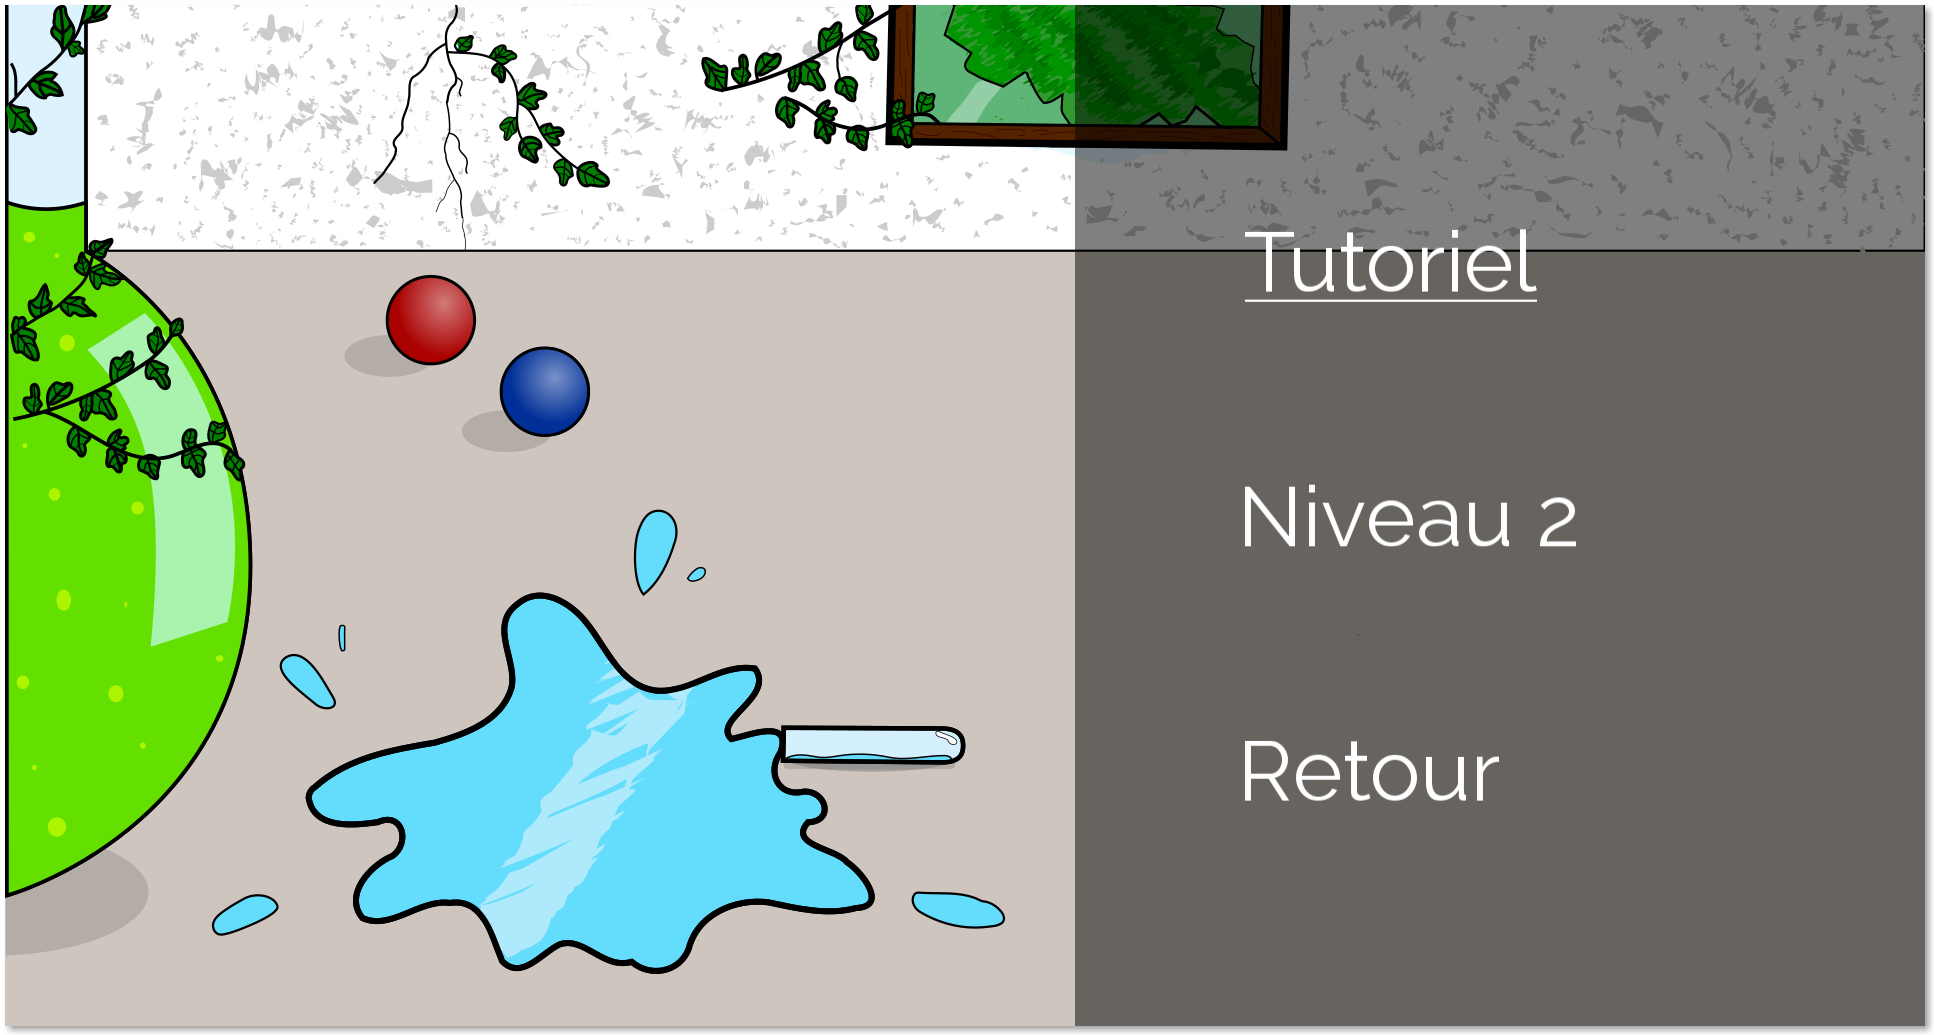
\includegraphics[width=13cm]{figures/menu_jouer.png}}
    \caption {Menu jouer}
    \label {fig:MJ}
\end{figure}

\noindent Ce menu [\ref{fig:MJ}] se compose de deux types de boutons : les boutons niveaux permettent aux joueurs de choisir un espace de jeu et
le bouton retour de revenir vers le menu principal [\ref{fig:MP}].\\

\begin {itemize}
\item \bf Le bouton règles du jeu.
\end {itemize}

Ce bouton affiche les règles du jeu.
\\
\\

\begin {itemize}
\item \bf Le bouton éditeur.
\end {itemize}

Ce bouton permet de créer un nouveau niveau ou de modifier un niveau existant.

\newpage

\begin{figure} [!h]
    \centerline {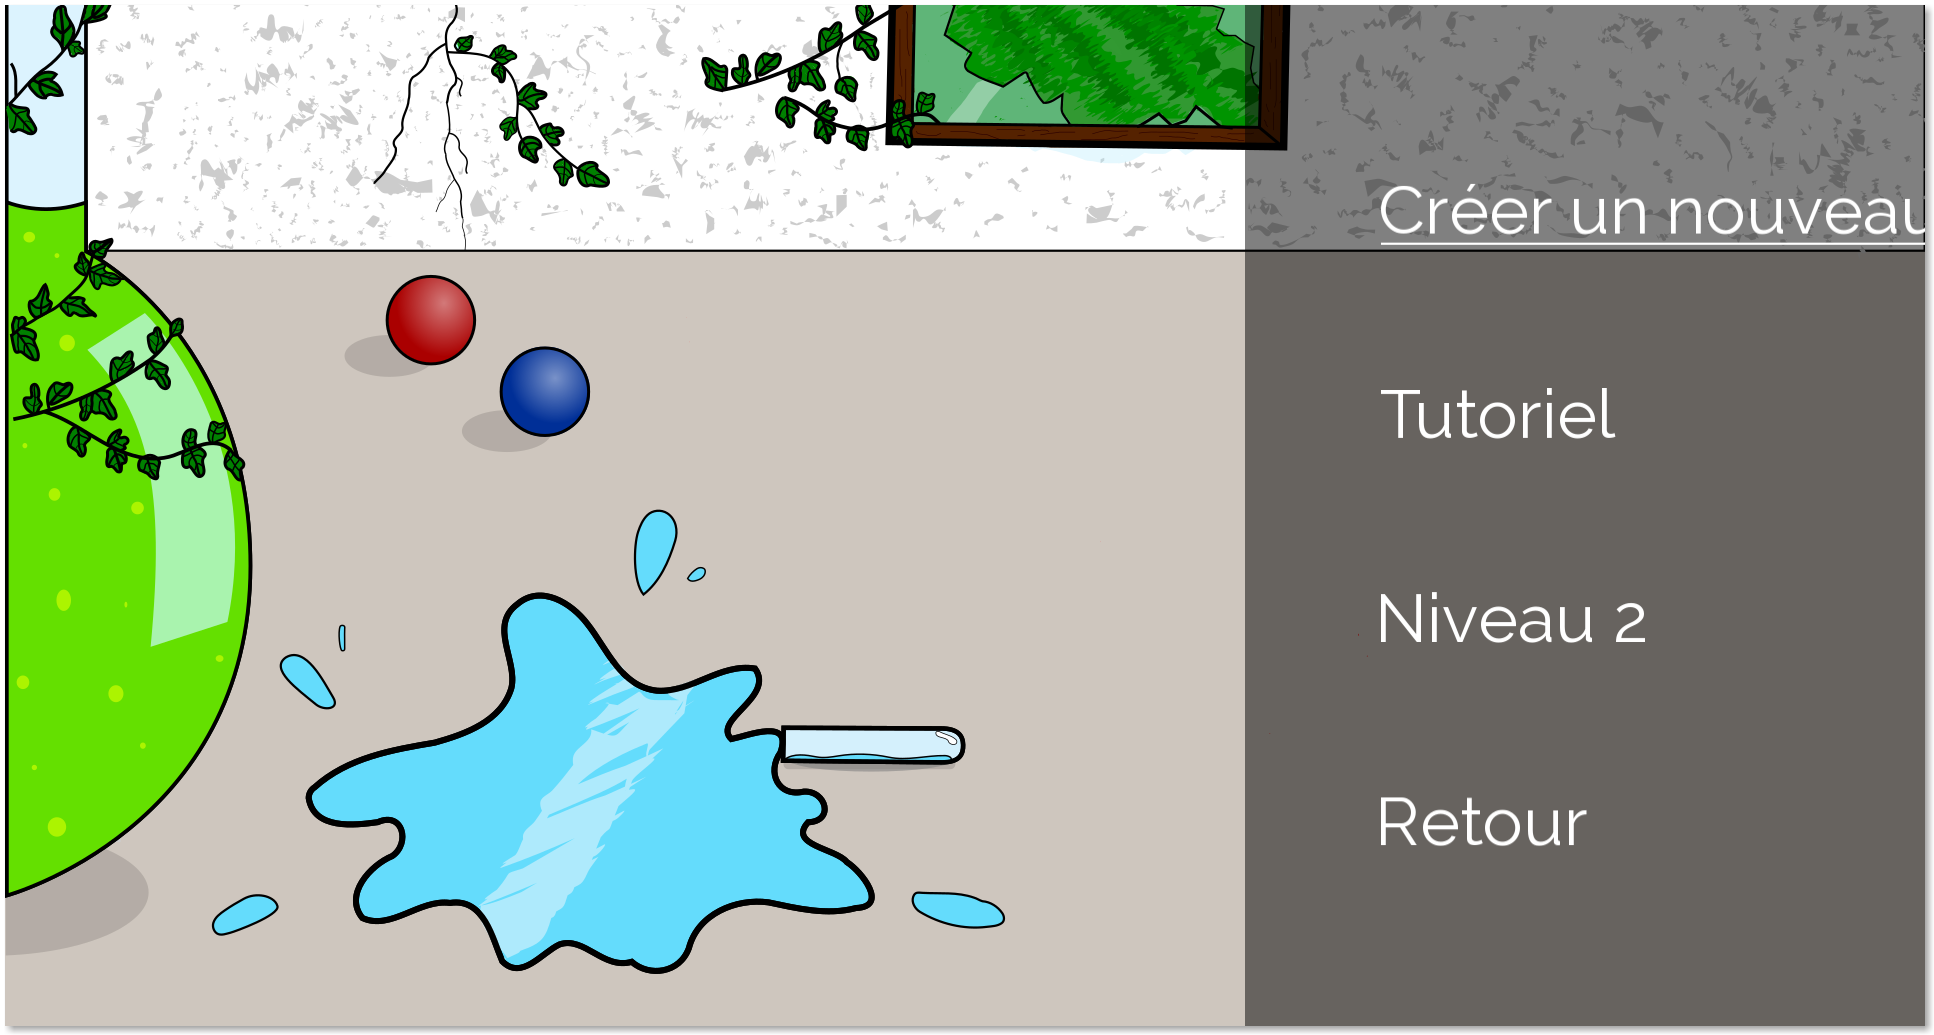
\includegraphics[width=13cm]{figures/menu_editeur.png}}
    \caption {Menu éditeur}
    \label {fig:ME}
\end{figure}


\noindent Ce menu [\ref{fig:ME}] se compose de trois types de boutons : Créer un nouveau niveau, éditer un niveau existant,
 et retour qui renvoie vers le menu principal [\ref{fig:MP}].\\




\noindent Les touches \Touche{$\uparrow$} , \Touche{$\downarrow$} ou
le passage de la souris sur un des boutons permettent la séléction d'un élément du menu.
le bouton sélectionné se souligne.\\

\noindent La touche \Touche{Enter} ou un clic avec la souris permettent de valider le choix.\\

\noindent Les touches \Touche{Backspace} et \Touche{Echap} permettent de revenir au menu précédent. \\

\subsection {Objets}

\label {OB}

\subsubsection{Balles}

\noindent {\raisebox{-.4\height}{
\includegraphics[width=23px]{figures/ball_1.png}} Les balles sont controlées par les joueurs. \\

\subsubsection{Polarité}

\noindent {\raisebox{-.4\height}{
\includegraphics[width=23px]{figures/block_blue.png}} Les objets de couleurs bleus repoussent tous ceux de la même couleur et attirent les objets de couleurs rouges. \\

\noindent {\raisebox{-.4\height}{
\includegraphics[width=23px]{figures/block_red.png}} Les objets de couleurs rouges repoussent tous ceux de la même couleur et attirent les objets de couleurs bleus. \\

\subsubsection{Blocs}

\noindent {\raisebox{-.4\height}{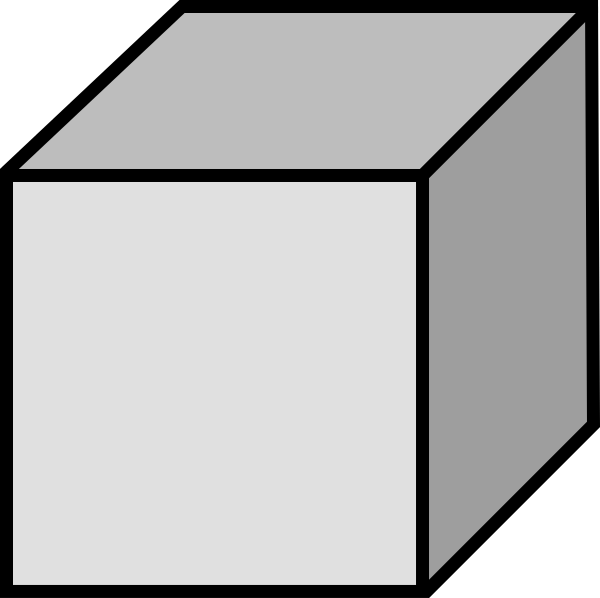
\includegraphics[width=23px]{figures/block.png}} Le bloc de base ne réalise aucune action particulière. \\

\noindent \raisebox{-.4\height}{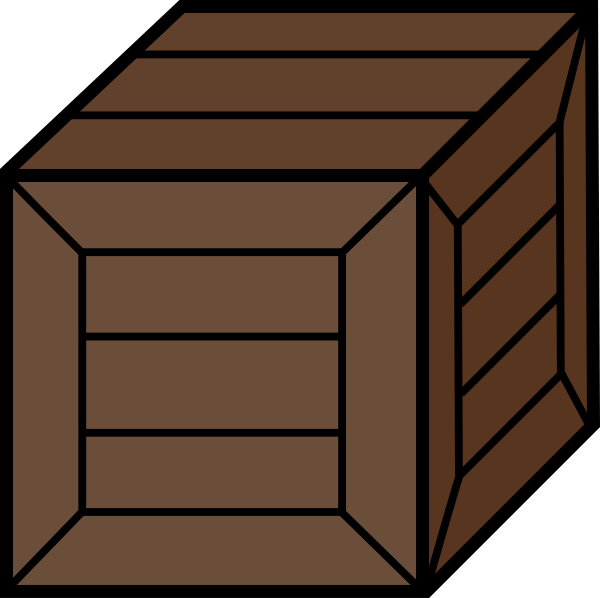
\includegraphics[width=23px]{figures/block_caisse.png}} La caisse est un bloc qui peut être poussé. \\

\noindent \raisebox{-.4\height}{
\includegraphics[width=23px]{figures/block_gravity_south.png}} Le bloc de gravité modifie le sens de la gravité lorsqu'un joueur ou une caisse rentre en collision avec lui. \\

\noindent \raisebox{-.4\height}{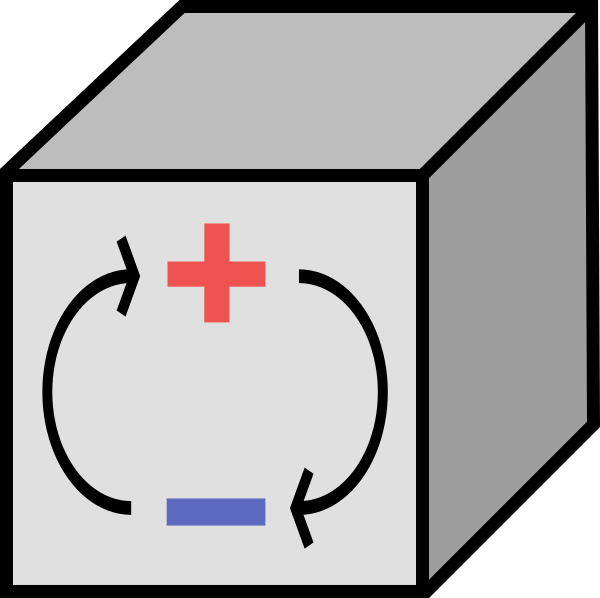
\includegraphics[width=23px]{figures/block_polarity.png}} Le bloc inverseur de polarité inverse la polarité de la balle qui rentre en collision avec lui. \\

\noindent \raisebox{-.4\height}{
\includegraphics[width=23px]{figures/block_dead.png}} Le bloc de mort fait perdre la partie si un des deux joueurs rentrent en collision avec lui. \\

\noindent \raisebox{-.3\height}{
\includegraphics[width=23px]{figures/block_end_2.png}} Le bloc d'arrivée fait gagner le joueur qui rentre en collision avec lui. \\


\subsection {Jeux}

\label {joué}

Les joueurs ne peuvent déplacer leurs balles que vers la gauche ou la droite.\\
Le joueur 1 utilise \Touche{$\rightarrow$} pour se déplacer vers la droite et \Touche{$\leftarrow$} pour se déplacer vers la gauche.\\
Le joueur 2 utilise \Touche{D} pour se déplacer vers la droite et \Touche{Q} pour se déplacer vers la gauche.\\

Les joueurs peuvent mettre le jeu en pause avec la touche \Touche{Échap}, ou bien quitter le niveau en appuyant sur \Touche{Espace}.

Un joueur peut mourrir de deux façons; soit en rentrant en collision avec un bloc de mort \raisebox{-.4\height}{
\includegraphics[width=15px]{figures/block_dead.png}} soit en sortant de la zone jouable.\\
\\

\subsection {Editeur}

\begin{figure} [!h]
    \centerline {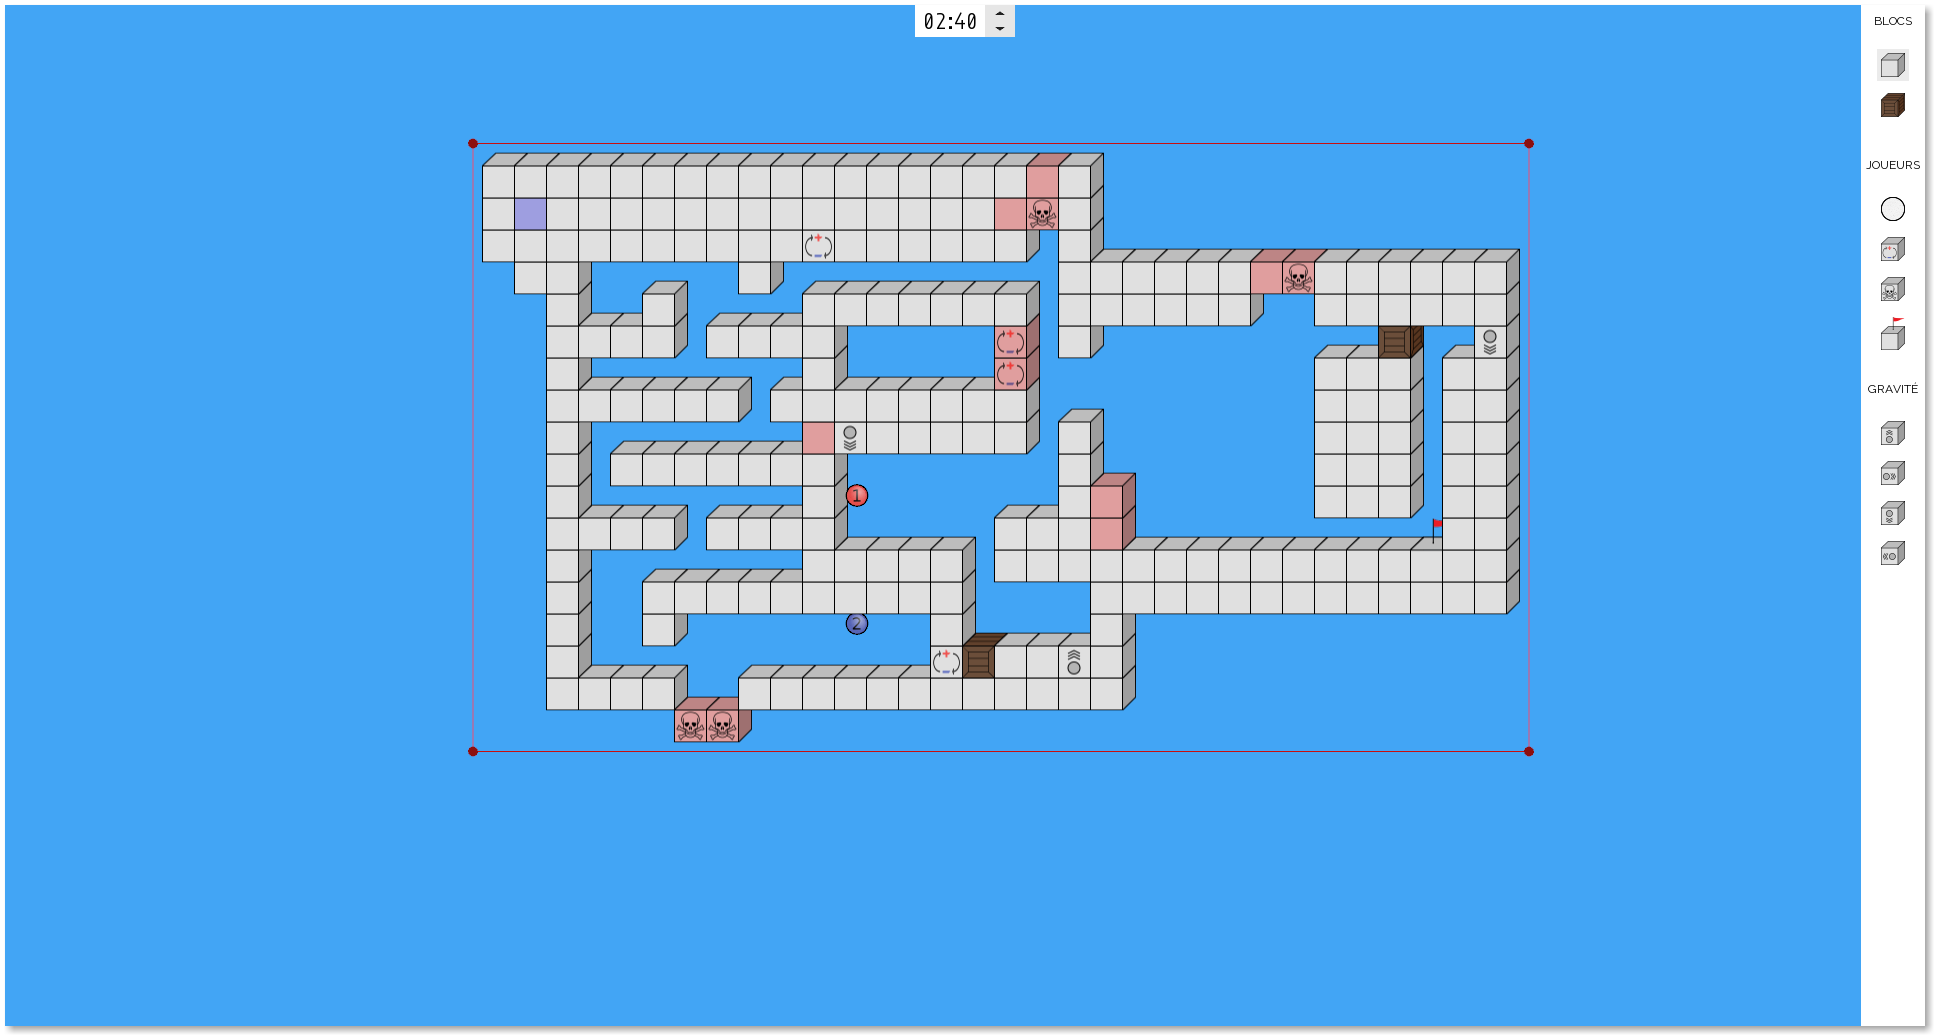
\includegraphics[width=13cm]{figures/editeur.png}}
    \caption {Éditeur}
    \label {fig:ED}
\end{figure}

\subsubsection {Gestion des objets}

La séléction de l'objet s'éffectue dans la barre latérale droite de la fenêtre à l'aide de la souris. [\ref{fig:ED}] \\
Un clic avec le bouton gauche de la souris permet de le placer sur un zone libre.
Le maintien du clic gauche permet de placer plusieurs objets à la fois.\\

Pour modifier la polarité d'un objet, le curseur doit être placé sur celui-ci. La touche \Touche{Ctrl} doit être enfoncée tout en faisant glisser la mollette de la souris, ou bien en faisant glisser deux doigts sur le pavé tactile vers le haut ou le bas. \\
\\

La selection d'un objet se fait avec la touche \Touche{Ctrl} et un clic sur celui-ci. Une multi-sélection peut être réalisée en cliquant sur plusieurs objets tout en maintenant la touche \Touche{Ctrl} enfoncée. \\
La réalisation d'une sélection rectangulaire est possible en maintenant la touche \Touche{Shift} et en faisant glisser la souris avec le clic gauche enfoncé sur la zone à sélectionner. \\
Un objet sélectionné a des bordures rouges. [\ref{fig:BBS}]\\

\begin{figure} [!h]
    \centerline {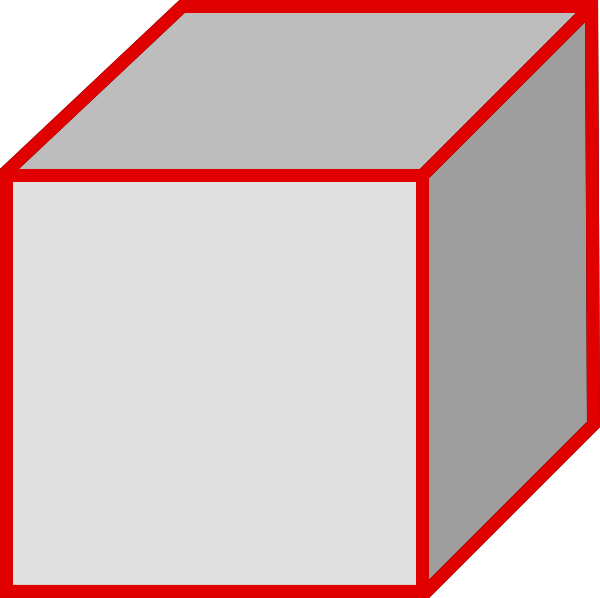
\includegraphics[width=25px]{figures/block_selection.png}}
    \caption {Bloc de base sélectionné}
    \label {fig:BBS}
\end{figure}

La suppression d'un objet s'effectue en cliquant dessus avec le bouton droit de la souris.
Plusieurs objets peuvent être supprimés aprés leurs séléctions en appuyant sur la touche \Touche{Suppr}.


\subsubsection {Compte à rebours}

Le compte à rebours se situe en haut au centre de le fenêtre. Durant la partie s'il arrive à 0, les joueurs meurent et la partie est perdue.\\

La valeur du compte à rebours peut être modifiée dans l'éditeur en cliquant sur les fléches se situant à coté.
Il est également possible de placer la souris sur ce dernier en faisant glisser la mollette ou deux doigts sur le pavé tactile vers le haut ou le bas. \\

\subsubsection {Zone de jeu}
La zone jouable est représentée dans l'éditeur par un polygone rouge [\ref{fig:ED}] composé de quatre points.
 Chacun de ces points peuvent être déplacés en cliquant dessus afin de modifier la taille et la forme de la zone.

\subsubsection {Gestion de la caméra}
Le déplacement de la caméra s'effectue en plaçant la souris vers une bordure de la fenêtre.
La molette de la souris peut être utilisée pour un défilement vertical ou horizontal si la touche \Touche{Shift} est enfoncée.
\\

il es possible également de faire glisser deux doigts sur le pavé tactile afin de déplacer la caméra dans la direction désirée.\\

\subsubsection {Commandes générales}

Il est possible de tester le niveau à tout moment en appuyant sur la touche \Touche{Espace}.
Pour revenir à l'édition il faut appuyer de nouveau sur \Touche{Espace}.\\
\\

Afin de sauvegarder le niveau il est necessaire de réaliser la combinaison de touches suivantes : \Touche{Ctrl} + \Touche {S}. (en mode édition).\\
\\

Pour quitter l’éditeur et revenir au menu la touche \Touche{Échap} doit être utilisé.

\chapter{Conclusion}

\section{Perspectives}
Par manque de temps, de nombreuses perspectives d'amélioration n'ont pas pu
aboutir. Nous aurions pu améliorer l'interface graphique (ce qui est prévu
avant l'oral), faire plus de niveaux et donc ajouter des musiques pour ces
nouveaux niveaux, ou encore ajouter les menus pause, victoire et défaite.

\section{Conclusions}

\subsection{Fonctionnement de l'application}

Nous avons remarqué qu'un message d'erreur « l'application ne répond pas »
s'affiche dans certaines circonstances que nous n'avons pas réussi à isoler,
bien que le programme réponde toujours.

Lors de la rotation de la caméra à la suite d'un changement dans la direction
de la gravité, la caméra ne réalise pas toujours le mouvement le plus rapide
et peut effectuer une rotation à 270 degrés au lieu de 90 degrés dans certaines
circonstances.

Dans certains cas les blocs déplaçables, si placés en trop grandes quantités,
se traversent. De plus, l'algorithme de collisions étant discret, un objet
ayant une vitesse trop élevée peut passer à travers un autre.

Enfin, la force d'attraction ne réagit pas tout à fait comme nous l'avions
imaginée initialement : elle est moins souple. Cela est probablement lié
à un mauvais ajustement dans les constantes du moteur physique. Cette
force fonctionne malgré tout.

Cependant, les menus ainsi que les retours aux menus fonctionnent bien,
l'affichage est fluide, l'éditeur est fonctionnel et comporte de nombreuses
fonctionnalités intuitives. Les ressources ne posent pas de problème,
les textures se chargent et les musiques se déclenchent correctement
et bouclent comme prévu.

Globalement, le jeu est fonctionnel et ne pose problème que dans des
cas très particuliers, il reste tout de même stable malgré le temps
limité que nous avions pour régler les problèmes.

\subsection{Fonctionnement du groupe de travail}

Le principal problème du groupe fut le sens des priorités. Nous nous sommes
attardés sur des détails avant que le tout soit fonctionnel, ce qui a
perturbé notre gestion du temps. Malgré cela, nous avons réussi à nous
organiser pour gagner en efficacité en partageant les tâches les plus
chronophages.

Le fait de refaire fréquemment le diagramme de Gantt nous a permis de
rattraper en partie le retard que nous avions pris. Au niveau de la
communication, nous n'avons eu aucun problème car nous nous
retrouvions très souvent sur Skype ainsi qu'à l'université afin
de discuter de tout problème et optimiser nos chances de trouver
rapidement une solution.

Malgré une gestion du temps perturbée, notre organisation et notre
communication nous ont permis de compenser les défauts du groupe,
et ainsi d'avancer à un rythme convenable.

Ainsi, grâce à notre détermination et notre coopération, nous avons
su franchir les difficultés et ainsi proposer un jeu fonctionnel et amusant.


% Bibliographie
\cleardoublepage
\phantomsection
\addcontentsline{toc}{chapter}{Webographie}
\bibliographystyle{unsrt}
\bibliography{rapport}

\end{document}
